\chapter{Implementation}\label{ch:implementation}

%\Todo{Here we can put pictures and codes snippets}\\

%Instead of having a huge amount of different pre-recorded sound files, which need a lot of space, we eliminate the problem to a \colorbox{pink}{2D look up}, where the algorithm matches the object first and then the exact point of the object that collided with some other object.
%

All synthetic sounds have been created in Pd patches and are interpreted by Heavy which generates audio plugins and a C\# interface for Unity. This C\# script is attached to the GameObject in the scene so that the sound is processed within the game world.

We have created our own script that assigns to every one of the objects  the modal parameters we extracted in the analysis part with the ChucK code. This is done independently of synthesis methods used here below.

\section{Impact Sounds}
%\Todo{decribe the patch, describe the sound (starts low, goes to max ampl and then decays etc)}\\
%\Todo{Put spectrogram pictures of the sounds to describe them}
%
\subsection{Sinusoidal Additive Synthesis}

In this section we describe in depth how the Pd patch corresponding to the sinusoidal additive synthesis of impact sounds works. The patch attempts to translate equation \ref{eq:modal_response} into the programming language of Pd. Some of its terms will be referenced in the following explanation.

First of all the frequencies and amplitudes matching the ten modes of the object are initialized. We can therefore feed these frequencies, which we identified as $f_n$ in the equation \ref{eq:modal_response}, into the different oscillators. In Pd, oscillators output a cosine wave which is equivalent to $cos(2 \pi f_nt)$ from the equation which suits our purpose perfectly.

We would also like to translate into Pd the expression $e^{-d_n t}$ which corresponds to the damping of every mode $n$. Gaver \cite{gaver1993we} states that for each partial the decay rates $d_n$ are controllable through a parameter $D$ which corresponds to a material and that a useful heuristic, that we use, is to have $d_n = 2 \pi f_nD$. By experimenting we established that values of $D$ range from approximately 0.0002 for metal to about 0.05 for plastic sounds, with glass, ceramic and wood sounds in between. The higher the damping the higher the values. Then we multiply the damping by the partial's initial amplitude $A_n$ to obtain an amplitude envelope that varies over time and which we multiply by the oscillator's signal. The output is what we call a partial. 

The final sound is produced by adding together the ten partials. The resulting signal is multiplied by the magnitude of the impact. \colorbox{pink}{For this we calculate the kinetic energy with Unity's physics components}. As described in \cite{farnell2010designing} before sending the signal to the DAC we pass it through a clipper that gives richer harmonics and produces brighter sounds the stronger the impact is.

The patch produces an impact sound whenever the OnCollisionEnter() method from Unity is called. This is done when the collider that has the script attached to it touches another collider. When this happens we set the magnitude of the collision and then send an event to excite the patch. This is done by setting the value of $t$ in \ref{eq:modal_response} to zero which increases over time making the sound decay.

\subsection{Filter-based Modal Synthesis}

For this synthesis method we will excite a bank of ten bandpass filters with an impulse signal to approximate a resonator.

The same way we did in the previous method, we initialize all ten frequencies and amplitudes of the object. Every frequency $f_n$ is sent into a bandpass filter as the center frequency. 

Every filter is characterized by its Q factor which is directly related to the damping. The value of Q will then determine the material of the impacted object.

To hit the object we use an impulse signal to excite the filter.
\begin{figure}[H]
  \centering
    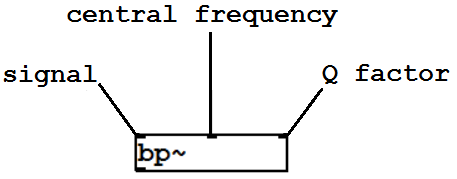
\includegraphics[width=0.5\textwidth]{bandpassfilter.png}
      \caption{Pd's bandpass filter with its three inlets, audio signal on the left, central frequency n the middle and Q factor on the right.}
      \label{fig:pot_sep}
\end{figure} 

\section{Rolling Sounds}

\section{Scratching Sounds}

\section{Assignment of Different Materials}
Different materials can be assigned to the objects made for this thesis. The designer is able to choose between \textit{plastic, wooden, ceramic, glass and metal} by adjusting a slider on the interface. 

Metallic or glass sounds are more ``ringy'' than wooden or plastic ones that are more ``thud''. We achieve those sounds by changing the \textbf{Q-factor} of the \textbf{band-pass filters} used in the pd patch. Q-factor indicated the power loss in the filter. The higher the Q the less power is lost, so the resonator vibrates longer \cite{bib:Q}.

\section{Changing the Size}
In an application, the same object can appear in different sizes, so this thesis takes this into account. It is known that under the same excitation, the smaller the size of an object, the more high pitched sounds it will produce, because the sound waves travel a smaller distance. Hence, we implemented a slider for the designer to choose the best sound that corresponds to the size of her object. 

\section{User Interface}
